\documentclass[12pt]{article}
\usepackage[margin=0.5cm, paperwidth=22cm, paperheight=16cm]{geometry}
\usepackage{tikz}
\usetikzlibrary{patterns, calc, arrows.meta, shapes.geometric, positioning}
\usepackage{varwidth}

\tikzset{
    sombreado/.style={fill=black!80},
}

\begin{document}

%%% PAGE 1 — Q4: cadena de óvalos
\begin{varwidth}{16cm}
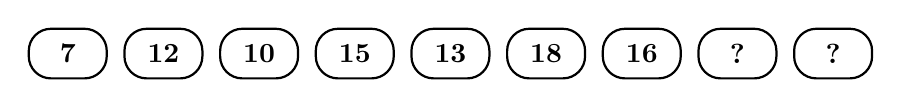
\begin{tikzpicture}[scale=0.9]
\foreach \i/\val in {0/7, 1/12, 2/10, 3/15, 4/13, 5/18, 6/16} {
    \draw[line width=0.8pt, rounded corners=8pt] (\i*1.35-0.55, -0.35) rectangle (\i*1.35+0.55, 0.35);
    \node at (\i*1.35, 0) {\textbf{\val}};
}
\foreach \i in {7, 8} {
    \draw[line width=0.8pt, rounded corners=8pt] (\i*1.35-0.55, -0.35) rectangle (\i*1.35+0.55, 0.35);
    \node at (\i*1.35, 0) {\textbf{?}};
}
\end{tikzpicture}
\end{varwidth}

\newpage

%%% PAGE 2 — Q5: cuadrícula serpentina (serie)
\begin{varwidth}{20cm}
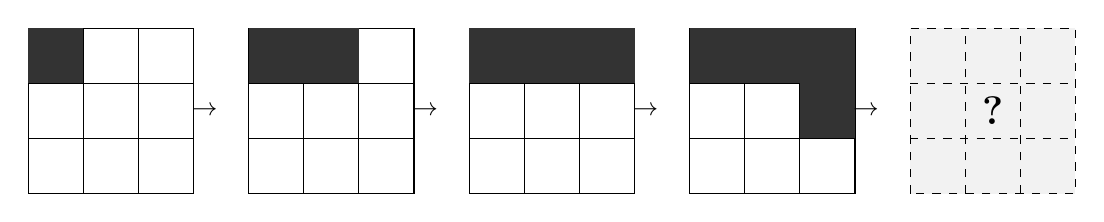
\begin{tikzpicture}[scale=0.7]
\begin{scope}[shift={(0,0)}]
\draw (0,0) grid (3,3);
\fill[sombreado] (0,2) rectangle (1,3);
\end{scope}
\begin{scope}[shift={(4,0)}]
\draw (0,0) grid (3,3);
\fill[sombreado] (0,2) rectangle (1,3);
\fill[sombreado] (1,2) rectangle (2,3);
\end{scope}
\begin{scope}[shift={(8,0)}]
\draw (0,0) grid (3,3);
\fill[sombreado] (0,2) rectangle (1,3);
\fill[sombreado] (1,2) rectangle (2,3);
\fill[sombreado] (2,2) rectangle (3,3);
\end{scope}
\begin{scope}[shift={(12,0)}]
\draw (0,0) grid (3,3);
\fill[sombreado] (0,2) rectangle (1,3);
\fill[sombreado] (1,2) rectangle (2,3);
\fill[sombreado] (2,2) rectangle (3,3);
\fill[sombreado] (2,1) rectangle (3,2);
\end{scope}
\begin{scope}[shift={(16,0)}]
\draw[dashed, fill=gray!10] (0,0) rectangle (3,3);
\draw[dashed] (1,0) -- (1,3);
\draw[dashed] (2,0) -- (2,3);
\draw[dashed] (0,1) -- (3,1);
\draw[dashed] (0,2) -- (3,2);
\node at (1.5,1.5) {\Large\textbf{?}};
\end{scope}
\foreach \x in {3.2, 7.2, 11.2, 15.2} {
    \node at (\x, 1.5) {\small$\rightarrow$};
}
\end{tikzpicture}

\bigskip

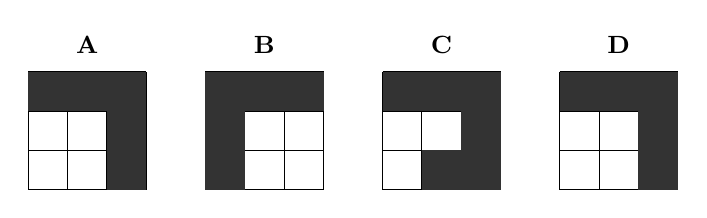
\begin{tikzpicture}[scale=0.5]
\begin{scope}[shift={(0,0)}]
\node[above] at (1.5,3.2) {\small\textbf{A}};
\draw (0,0) grid (3,3);
\fill[sombreado] (0,2) rectangle (1,3);
\fill[sombreado] (1,2) rectangle (2,3);
\fill[sombreado] (2,2) rectangle (3,3);
\fill[sombreado] (2,1) rectangle (3,2);
\fill[sombreado] (2,0) rectangle (3,1);
\end{scope}
\begin{scope}[shift={(4.5,0)}]
\node[above] at (1.5,3.2) {\small\textbf{B}};
\draw (0,0) grid (3,3);
\fill[sombreado] (0,2) rectangle (1,3);
\fill[sombreado] (1,2) rectangle (2,3);
\fill[sombreado] (2,2) rectangle (3,3);
\fill[sombreado] (0,1) rectangle (1,2);
\fill[sombreado] (0,0) rectangle (1,1);
\end{scope}
\begin{scope}[shift={(9,0)}]
\node[above] at (1.5,3.2) {\small\textbf{C}};
\draw (0,0) grid (3,3);
\fill[sombreado] (0,2) rectangle (3,3);
\fill[sombreado] (2,1) rectangle (3,2);
\fill[sombreado] (1,0) rectangle (3,1);
\end{scope}
\begin{scope}[shift={(13.5,0)}]
\node[above] at (1.5,3.2) {\small\textbf{D}};
\draw (0,0) grid (3,3);
\fill[sombreado] (0,2) rectangle (3,3);
\fill[sombreado] (2,0) rectangle (3,2);
\end{scope}
\end{tikzpicture}
\end{varwidth}

\newpage

%%% PAGE 3 — Q6: cuadrado + punto + lado grueso (serie)
\begin{varwidth}{18cm}
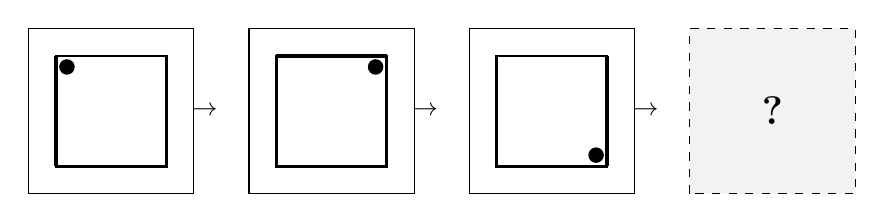
\begin{tikzpicture}[scale=0.7]
% Cuadro 1
\begin{scope}[shift={(0,0)}]
\draw[line width=0.5pt] (0,0) rectangle (3,3);
\draw[line width=1pt] (0.5,0.5) rectangle (2.5,2.5);
\fill (0.7,2.3) circle (4pt);
\draw[line width=1.5pt] (0.5,0.5) -- (0.5,2.5);
\end{scope}
% Cuadro 2
\begin{scope}[shift={(4,0)}]
\draw[line width=0.5pt] (0,0) rectangle (3,3);
\draw[line width=1pt] (0.5,0.5) rectangle (2.5,2.5);
\fill (2.3,2.3) circle (4pt);
\draw[line width=1.5pt] (0.5,2.5) -- (2.5,2.5);
\end{scope}
% Cuadro 3
\begin{scope}[shift={(8,0)}]
\draw[line width=0.5pt] (0,0) rectangle (3,3);
\draw[line width=1pt] (0.5,0.5) rectangle (2.5,2.5);
\fill (2.3,0.7) circle (4pt);
\draw[line width=1.5pt] (2.5,0.5) -- (2.5,2.5);
\end{scope}
% Cuadro 4: ?
\begin{scope}[shift={(12,0)}]
\draw[dashed, fill=gray!10] (0,0) rectangle (3,3);
\node at (1.5,1.5) {\Large\textbf{?}};
\end{scope}
\foreach \x in {3.2, 7.2, 11.2} {
    \node at (\x, 1.5) {\small$\rightarrow$};
}
\end{tikzpicture}

\bigskip

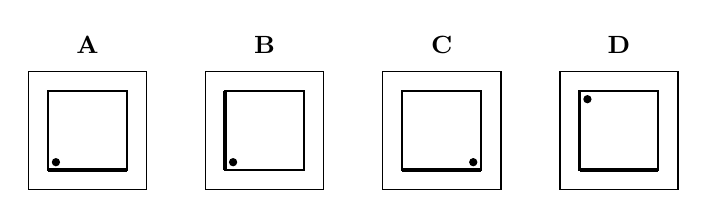
\begin{tikzpicture}[scale=0.5]
\begin{scope}[shift={(0,0)}]
\node[above] at (1.5,3.2) {\small\textbf{A}};
\draw[line width=0.5pt] (0,0) rectangle (3,3);
\draw[line width=0.8pt] (0.5,0.5) rectangle (2.5,2.5);
\fill (0.7,0.7) circle (3pt);
\draw[line width=1.5pt] (0.5,0.5) -- (2.5,0.5);
\end{scope}
\begin{scope}[shift={(4.5,0)}]
\node[above] at (1.5,3.2) {\small\textbf{B}};
\draw[line width=0.5pt] (0,0) rectangle (3,3);
\draw[line width=0.8pt] (0.5,0.5) rectangle (2.5,2.5);
\fill (0.7,0.7) circle (3pt);
\draw[line width=1.5pt] (0.5,0.5) -- (0.5,2.5);
\end{scope}
\begin{scope}[shift={(9,0)}]
\node[above] at (1.5,3.2) {\small\textbf{C}};
\draw[line width=0.5pt] (0,0) rectangle (3,3);
\draw[line width=0.8pt] (0.5,0.5) rectangle (2.5,2.5);
\fill (2.3,0.7) circle (3pt);
\draw[line width=1.5pt] (0.5,0.5) -- (2.5,0.5);
\end{scope}
\begin{scope}[shift={(13.5,0)}]
\node[above] at (1.5,3.2) {\small\textbf{D}};
\draw[line width=0.5pt] (0,0) rectangle (3,3);
\draw[line width=0.8pt] (0.5,0.5) rectangle (2.5,2.5);
\fill (0.7,2.3) circle (3pt);
\draw[line width=1.5pt] (0.5,0.5) -- (2.5,0.5);
\end{scope}
\end{tikzpicture}
\end{varwidth}

\newpage

%%% PAGE 4 — Q7: círculos con sectores
\begin{varwidth}{18cm}
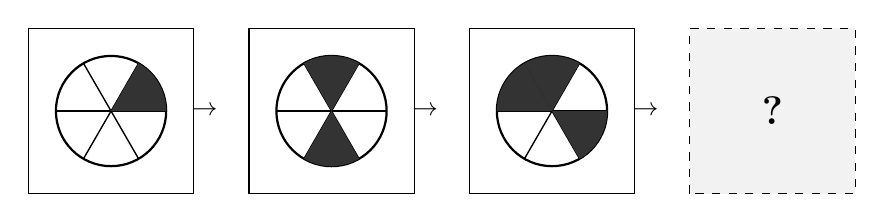
\begin{tikzpicture}[scale=0.7]
% Cuadro 1: 1 sector
\begin{scope}[shift={(0,0)}]
\draw[line width=0.5pt] (0,0) rectangle (3,3);
\draw[line width=0.8pt] (1.5,1.5) circle (1);
\foreach \a in {0,60,...,300} {
    \draw[line width=0.5pt] (1.5,1.5) -- ({1.5+1*cos(\a)},{1.5+1*sin(\a)});
}
\fill[sombreado] (1.5,1.5) -- ({1.5+1*cos(0)},{1.5+1*sin(0)}) arc (0:60:1) -- cycle;
\end{scope}
% Cuadro 2: 2 sectores opuestos
\begin{scope}[shift={(4,0)}]
\draw[line width=0.5pt] (0,0) rectangle (3,3);
\draw[line width=0.8pt] (1.5,1.5) circle (1);
\foreach \a in {0,60,...,300} {
    \draw[line width=0.5pt] (1.5,1.5) -- ({1.5+1*cos(\a)},{1.5+1*sin(\a)});
}
\fill[sombreado] (1.5,1.5) -- ({1.5+1*cos(60)},{1.5+1*sin(60)}) arc (60:120:1) -- cycle;
\fill[sombreado] (1.5,1.5) -- ({1.5+1*cos(240)},{1.5+1*sin(240)}) arc (240:300:1) -- cycle;
\end{scope}
% Cuadro 3: 3 sectores
\begin{scope}[shift={(8,0)}]
\draw[line width=0.5pt] (0,0) rectangle (3,3);
\draw[line width=0.8pt] (1.5,1.5) circle (1);
\foreach \a in {0,60,...,300} {
    \draw[line width=0.5pt] (1.5,1.5) -- ({1.5+1*cos(\a)},{1.5+1*sin(\a)});
}
\fill[sombreado] (1.5,1.5) -- ({1.5+1*cos(120)},{1.5+1*sin(120)}) arc (120:180:1) -- cycle;
\fill[sombreado] (1.5,1.5) -- ({1.5+1*cos(300)},{1.5+1*sin(300)}) arc (300:360:1) -- cycle;
\fill[sombreado] (1.5,1.5) -- ({1.5+1*cos(60)},{1.5+1*sin(60)}) arc (60:120:1) -- cycle;
\end{scope}
% Cuadro 4: ?
\begin{scope}[shift={(12,0)}]
\draw[dashed, fill=gray!10] (0,0) rectangle (3,3);
\node at (1.5,1.5) {\Large\textbf{?}};
\end{scope}
\foreach \x in {3.2, 7.2, 11.2} {
    \node at (\x, 1.5) {\small$\rightarrow$};
}
\end{tikzpicture}

\bigskip

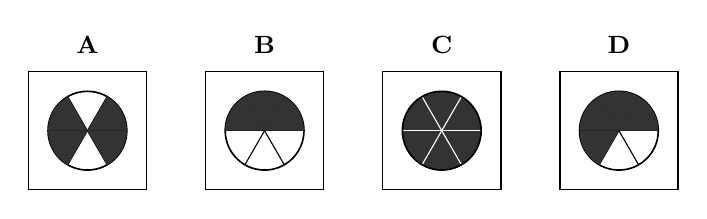
\begin{tikzpicture}[scale=0.5]
% A
\begin{scope}[shift={(0,0)}]
\node[above] at (1.5,3.2) {\small\textbf{A}};
\draw[line width=0.5pt] (0,0) rectangle (3,3);
\draw[line width=0.6pt] (1.5,1.5) circle (1);
\foreach \a in {0,60,...,300} {
    \draw[line width=0.4pt] (1.5,1.5) -- ({1.5+1*cos(\a)},{1.5+1*sin(\a)});
}
\fill[sombreado] (1.5,1.5) -- ({1.5+1*cos(180)},{1.5+1*sin(180)}) arc (180:240:1) -- cycle;
\fill[sombreado] (1.5,1.5) -- ({1.5+1*cos(0)},{1.5+1*sin(0)}) arc (0:60:1) -- cycle;
\fill[sombreado] (1.5,1.5) -- ({1.5+1*cos(120)},{1.5+1*sin(120)}) arc (120:180:1) -- cycle;
\fill[sombreado] (1.5,1.5) -- ({1.5+1*cos(300)},{1.5+1*sin(300)}) arc (300:360:1) -- cycle;
\end{scope}
% B
\begin{scope}[shift={(4.5,0)}]
\node[above] at (1.5,3.2) {\small\textbf{B}};
\draw[line width=0.5pt] (0,0) rectangle (3,3);
\draw[line width=0.6pt] (1.5,1.5) circle (1);
\foreach \a in {0,60,...,300} {
    \draw[line width=0.4pt] (1.5,1.5) -- ({1.5+1*cos(\a)},{1.5+1*sin(\a)});
}
\fill[sombreado] (1.5,1.5) -- ({1.5+1*cos(0)},{1.5+1*sin(0)}) arc (0:60:1) -- cycle;
\fill[sombreado] (1.5,1.5) -- ({1.5+1*cos(60)},{1.5+1*sin(60)}) arc (60:120:1) -- cycle;
\fill[sombreado] (1.5,1.5) -- ({1.5+1*cos(120)},{1.5+1*sin(120)}) arc (120:180:1) -- cycle;
\end{scope}
% C
\begin{scope}[shift={(9,0)}]
\node[above] at (1.5,3.2) {\small\textbf{C}};
\draw[line width=0.5pt] (0,0) rectangle (3,3);
\fill[sombreado] (1.5,1.5) circle (1);
\foreach \a in {0,60,...,300} {
    \draw[white, line width=0.4pt] (1.5,1.5) -- ({1.5+1*cos(\a)},{1.5+1*sin(\a)});
}
\draw[line width=0.6pt] (1.5,1.5) circle (1);
\end{scope}
% D
\begin{scope}[shift={(13.5,0)}]
\node[above] at (1.5,3.2) {\small\textbf{D}};
\draw[line width=0.5pt] (0,0) rectangle (3,3);
\draw[line width=0.6pt] (1.5,1.5) circle (1);
\foreach \a in {0,60,...,300} {
    \draw[line width=0.4pt] (1.5,1.5) -- ({1.5+1*cos(\a)},{1.5+1*sin(\a)});
}
\fill[sombreado] (1.5,1.5) -- ({1.5+1*cos(0)},{1.5+1*sin(0)}) arc (0:60:1) -- cycle;
\fill[sombreado] (1.5,1.5) -- ({1.5+1*cos(60)},{1.5+1*sin(60)}) arc (60:120:1) -- cycle;
\fill[sombreado] (1.5,1.5) -- ({1.5+1*cos(120)},{1.5+1*sin(120)}) arc (120:180:1) -- cycle;
\fill[sombreado] (1.5,1.5) -- ({1.5+1*cos(180)},{1.5+1*sin(180)}) arc (180:240:1) -- cycle;
\end{scope}
\end{tikzpicture}
\end{varwidth}

\newpage

%%% PAGE 5 — Q8: polígonos inscritos (serie) — CUADRADO CENTRADO
\begin{varwidth}{18cm}
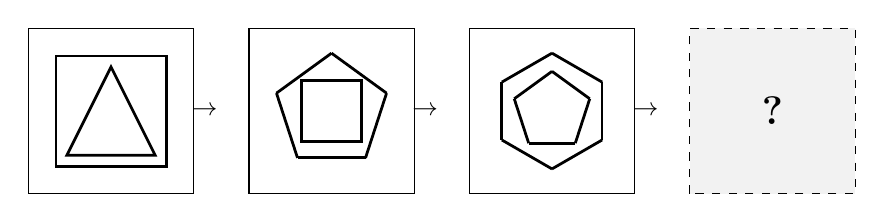
\begin{tikzpicture}[scale=0.7]
% Cuadro 1: triángulo en cuadrado
\begin{scope}[shift={(0,0)}]
\draw[line width=0.5pt] (0,0) rectangle (3,3);
\draw[line width=1pt] (0.5,0.5) rectangle (2.5,2.5);
\draw[line width=1pt] (1.5,2.3) -- (0.7,0.7) -- (2.3,0.7) -- cycle;
\end{scope}
% Cuadro 2: cuadrado en pentágono — CENTRADO
\begin{scope}[shift={(4,0)}]
\draw[line width=0.5pt] (0,0) rectangle (3,3);
\foreach \i in {0,...,4} {
    \draw[line width=1pt] ({1.5+1.05*cos(90+\i*72)},{1.5+1.05*sin(90+\i*72)}) -- ({1.5+1.05*cos(90+(\i+1)*72)},{1.5+1.05*sin(90+(\i+1)*72)});
}
\draw[line width=1pt] (0.95,0.95) rectangle (2.05,2.05);
\end{scope}
% Cuadro 3: pentágono en hexágono
\begin{scope}[shift={(8,0)}]
\draw[line width=0.5pt] (0,0) rectangle (3,3);
\foreach \i in {0,...,5} {
    \draw[line width=1pt] ({1.5+1.05*cos(30+\i*60)},{1.5+1.05*sin(30+\i*60)}) -- ({1.5+1.05*cos(30+(\i+1)*60)},{1.5+1.05*sin(30+(\i+1)*60)});
}
\foreach \i in {0,...,4} {
    \draw[line width=1pt] ({1.5+0.72*cos(90+\i*72)},{1.5+0.72*sin(90+\i*72)}) -- ({1.5+0.72*cos(90+(\i+1)*72)},{1.5+0.72*sin(90+(\i+1)*72)});
}
\end{scope}
% Cuadro 4: ?
\begin{scope}[shift={(12,0)}]
\draw[dashed, fill=gray!10] (0,0) rectangle (3,3);
\node at (1.5,1.5) {\Large\textbf{?}};
\end{scope}
\foreach \x in {3.2, 7.2, 11.2} {
    \node at (\x, 1.5) {\small$\rightarrow$};
}
\end{tikzpicture}

\bigskip

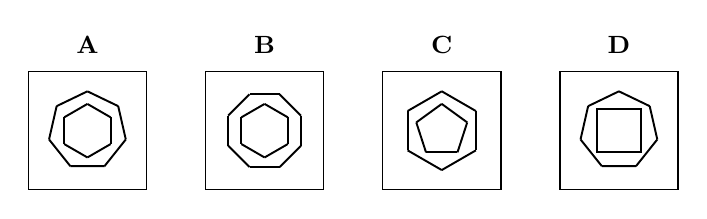
\begin{tikzpicture}[scale=0.5]
% A: hexágono en heptágono
\begin{scope}[shift={(0,0)}]
\node[above] at (1.5,3.2) {\small\textbf{A}};
\draw[line width=0.5pt] (0,0) rectangle (3,3);
\foreach \i in {0,...,6} {
    \draw[line width=0.7pt] ({1.5+1*cos(90+\i*51.43)},{1.5+1*sin(90+\i*51.43)}) -- ({1.5+1*cos(90+(\i+1)*51.43)},{1.5+1*sin(90+(\i+1)*51.43)});
}
\foreach \i in {0,...,5} {
    \draw[line width=0.7pt] ({1.5+0.68*cos(30+\i*60)},{1.5+0.68*sin(30+\i*60)}) -- ({1.5+0.68*cos(30+(\i+1)*60)},{1.5+0.68*sin(30+(\i+1)*60)});
}
\end{scope}
% B: hexágono en octágono
\begin{scope}[shift={(4.5,0)}]
\node[above] at (1.5,3.2) {\small\textbf{B}};
\draw[line width=0.5pt] (0,0) rectangle (3,3);
\foreach \i in {0,...,7} {
    \draw[line width=0.7pt] ({1.5+1*cos(22.5+\i*45)},{1.5+1*sin(22.5+\i*45)}) -- ({1.5+1*cos(22.5+(\i+1)*45)},{1.5+1*sin(22.5+(\i+1)*45)});
}
\foreach \i in {0,...,5} {
    \draw[line width=0.7pt] ({1.5+0.68*cos(30+\i*60)},{1.5+0.68*sin(30+\i*60)}) -- ({1.5+0.68*cos(30+(\i+1)*60)},{1.5+0.68*sin(30+(\i+1)*60)});
}
\end{scope}
% C: pentágono en hexágono (repetido)
\begin{scope}[shift={(9,0)}]
\node[above] at (1.5,3.2) {\small\textbf{C}};
\draw[line width=0.5pt] (0,0) rectangle (3,3);
\foreach \i in {0,...,5} {
    \draw[line width=0.7pt] ({1.5+1*cos(30+\i*60)},{1.5+1*sin(30+\i*60)}) -- ({1.5+1*cos(30+(\i+1)*60)},{1.5+1*sin(30+(\i+1)*60)});
}
\foreach \i in {0,...,4} {
    \draw[line width=0.7pt] ({1.5+0.68*cos(90+\i*72)},{1.5+0.68*sin(90+\i*72)}) -- ({1.5+0.68*cos(90+(\i+1)*72)},{1.5+0.68*sin(90+(\i+1)*72)});
}
\end{scope}
% D: cuadrado en heptágono
\begin{scope}[shift={(13.5,0)}]
\node[above] at (1.5,3.2) {\small\textbf{D}};
\draw[line width=0.5pt] (0,0) rectangle (3,3);
\foreach \i in {0,...,6} {
    \draw[line width=0.7pt] ({1.5+1*cos(90+\i*51.43)},{1.5+1*sin(90+\i*51.43)}) -- ({1.5+1*cos(90+(\i+1)*51.43)},{1.5+1*sin(90+(\i+1)*51.43)});
}
\draw[line width=0.7pt] (0.95,0.95) rectangle (2.05,2.05);
\end{scope}
\end{tikzpicture}
\end{varwidth}

\newpage

%%% PAGE 6 — Q9: conteo de triángulos
\begin{varwidth}{8cm}
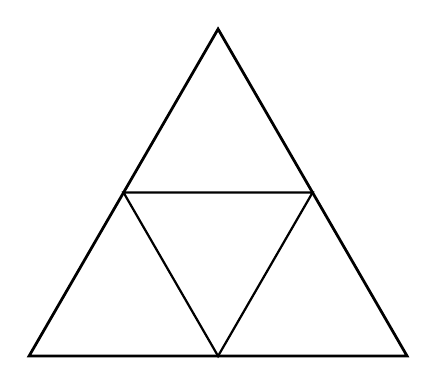
\begin{tikzpicture}[scale=1.2]
\coordinate (A) at (0,0);
\coordinate (B) at (4,0);
\coordinate (C) at (2,3.46);
\coordinate (AB) at (2,0);
\coordinate (AC) at (1,1.73);
\coordinate (BC) at (3,1.73);
\draw[line width=1pt] (A) -- (B) -- (C) -- cycle;
\draw[line width=0.8pt] (AB) -- (AC) -- (BC) -- cycle;
\end{tikzpicture}
\end{varwidth}

\newpage

%%% PAGE 7 — Q10: conteo de rectángulos
\begin{varwidth}{8cm}
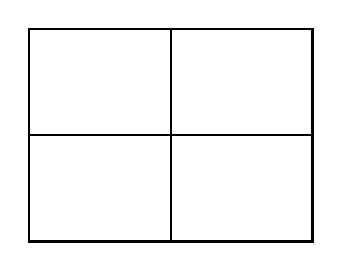
\begin{tikzpicture}[scale=0.9]
\draw[line width=1pt] (0,0) rectangle (4,3);
\draw[line width=0.8pt] (2,0) -- (2,3);
\draw[line width=0.8pt] (0,1.5) -- (4,1.5);
\end{tikzpicture}
\end{varwidth}

\newpage

%%% PAGE 8 — Q11: rotación de L (figura + opciones)
\begin{varwidth}{18cm}
\begin{center}
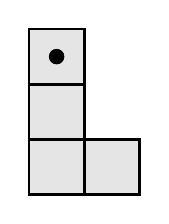
\begin{tikzpicture}[scale=0.7]
% Figura original
\draw[line width=1pt, fill=gray!20] (0,0) rectangle (1,1);
\draw[line width=1pt, fill=gray!20] (1,0) rectangle (2,1);
\draw[line width=1pt, fill=gray!20] (0,1) rectangle (1,2);
\draw[line width=1pt, fill=gray!20] (0,2) rectangle (1,3);
\fill (0.5, 2.5) circle (4pt);
\end{tikzpicture}
\end{center}

\bigskip

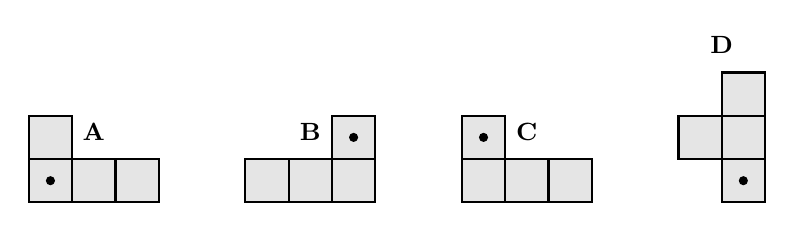
\begin{tikzpicture}[scale=0.55]
% A
\begin{scope}[shift={(0,0)}]
\node[above] at (1.5,1.2) {\small\textbf{A}};
\draw[line width=0.8pt, fill=gray!20] (0,0) rectangle (1,1);
\draw[line width=0.8pt, fill=gray!20] (1,0) rectangle (2,1);
\draw[line width=0.8pt, fill=gray!20] (2,0) rectangle (3,1);
\draw[line width=0.8pt, fill=gray!20] (0,1) rectangle (1,2);
\fill (0.5, 0.5) circle (3pt);
\end{scope}
% B
\begin{scope}[shift={(5,0)}]
\node[above] at (1.5,1.2) {\small\textbf{B}};
\draw[line width=0.8pt, fill=gray!20] (0,0) rectangle (1,1);
\draw[line width=0.8pt, fill=gray!20] (1,0) rectangle (2,1);
\draw[line width=0.8pt, fill=gray!20] (2,0) rectangle (3,1);
\draw[line width=0.8pt, fill=gray!20] (2,1) rectangle (3,2);
\fill (2.5, 1.5) circle (3pt);
\end{scope}
% C
\begin{scope}[shift={(10,0)}]
\node[above] at (1.5,1.2) {\small\textbf{C}};
\draw[line width=0.8pt, fill=gray!20] (0,0) rectangle (1,1);
\draw[line width=0.8pt, fill=gray!20] (1,0) rectangle (2,1);
\draw[line width=0.8pt, fill=gray!20] (2,0) rectangle (3,1);
\draw[line width=0.8pt, fill=gray!20] (0,1) rectangle (1,2);
\fill (0.5, 1.5) circle (3pt);
\end{scope}
% D
\begin{scope}[shift={(15,0)}]
\node[above] at (1,3.2) {\small\textbf{D}};
\draw[line width=0.8pt, fill=gray!20] (0,1) rectangle (1,2);
\draw[line width=0.8pt, fill=gray!20] (1,1) rectangle (2,2);
\draw[line width=0.8pt, fill=gray!20] (1,2) rectangle (2,3);
\draw[line width=0.8pt, fill=gray!20] (1,0) rectangle (2,1);
\fill (1.5, 0.5) circle (3pt);
\end{scope}
\end{tikzpicture}
\end{varwidth}

\newpage

%%% PAGE 9 — Q12: rotación 180° de T (figura + opciones)
\begin{varwidth}{18cm}
\begin{center}
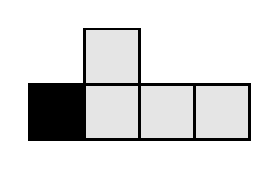
\begin{tikzpicture}[scale=0.7]
\draw[line width=1pt, fill=gray!20] (0,0) rectangle (1,1);
\draw[line width=1pt, fill=gray!20] (1,0) rectangle (2,1);
\draw[line width=1pt, fill=gray!20] (2,0) rectangle (3,1);
\draw[line width=1pt, fill=gray!20] (3,0) rectangle (4,1);
\draw[line width=1pt, fill=gray!20] (1,1) rectangle (2,2);
\fill[black] (0,0) rectangle (1,1);
\draw[line width=1pt] (0,0) rectangle (1,1);
\end{tikzpicture}
\end{center}

\bigskip

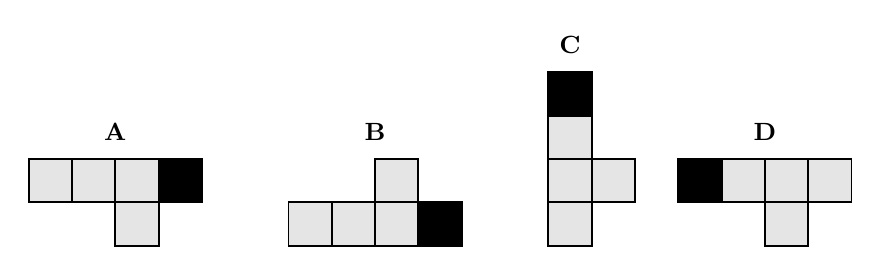
\begin{tikzpicture}[scale=0.55]
% A
\begin{scope}[shift={(0,0)}]
\node[above] at (2,2.2) {\small\textbf{A}};
\draw[line width=0.7pt, fill=gray!20] (0,1) rectangle (1,2);
\draw[line width=0.7pt, fill=gray!20] (1,1) rectangle (2,2);
\draw[line width=0.7pt, fill=gray!20] (2,1) rectangle (3,2);
\draw[line width=0.7pt, fill=gray!20] (3,1) rectangle (4,2);
\draw[line width=0.7pt, fill=gray!20] (2,0) rectangle (3,1);
\fill[black] (3,1) rectangle (4,2);
\draw[line width=0.7pt] (3,1) rectangle (4,2);
\end{scope}
% B
\begin{scope}[shift={(6,0)}]
\node[above] at (2,2.2) {\small\textbf{B}};
\draw[line width=0.7pt, fill=gray!20] (0,0) rectangle (1,1);
\draw[line width=0.7pt, fill=gray!20] (1,0) rectangle (2,1);
\draw[line width=0.7pt, fill=gray!20] (2,0) rectangle (3,1);
\draw[line width=0.7pt, fill=gray!20] (3,0) rectangle (4,1);
\draw[line width=0.7pt, fill=gray!20] (2,1) rectangle (3,2);
\fill[black] (3,0) rectangle (4,1);
\draw[line width=0.7pt] (3,0) rectangle (4,1);
\end{scope}
% C
\begin{scope}[shift={(12,0)}]
\node[above] at (0.5,4.2) {\small\textbf{C}};
\draw[line width=0.7pt, fill=gray!20] (0,0) rectangle (1,1);
\draw[line width=0.7pt, fill=gray!20] (0,1) rectangle (1,2);
\draw[line width=0.7pt, fill=gray!20] (0,2) rectangle (1,3);
\draw[line width=0.7pt, fill=gray!20] (0,3) rectangle (1,4);
\draw[line width=0.7pt, fill=gray!20] (1,1) rectangle (2,2);
\fill[black] (0,3) rectangle (1,4);
\draw[line width=0.7pt] (0,3) rectangle (1,4);
\end{scope}
% D
\begin{scope}[shift={(15,0)}]
\node[above] at (2,2.2) {\small\textbf{D}};
\draw[line width=0.7pt, fill=gray!20] (0,1) rectangle (1,2);
\draw[line width=0.7pt, fill=gray!20] (1,1) rectangle (2,2);
\draw[line width=0.7pt, fill=gray!20] (2,1) rectangle (3,2);
\draw[line width=0.7pt, fill=gray!20] (3,1) rectangle (4,2);
\draw[line width=0.7pt, fill=gray!20] (2,0) rectangle (3,1);
\fill[black] (0,1) rectangle (1,2);
\draw[line width=0.7pt] (0,1) rectangle (1,2);
\end{scope}
\end{tikzpicture}
\end{varwidth}

\newpage

%%% PAGE 10 — Q13: triángulos con números
\begin{varwidth}{14cm}
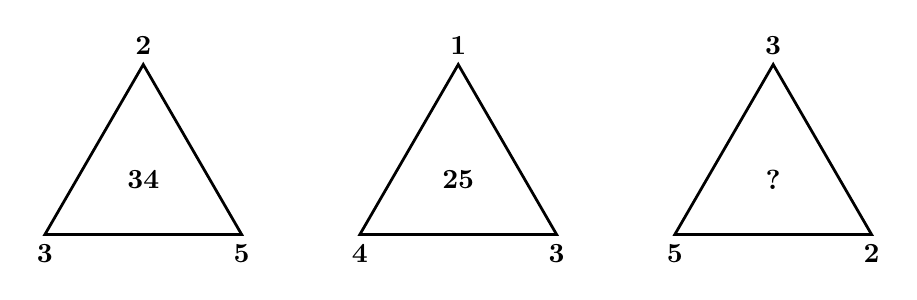
\begin{tikzpicture}[scale=1]
% Triángulo 1
\begin{scope}[shift={(0,0)}]
\draw[line width=1pt] (0,0) -- (2.5,0) -- (1.25,2.16) -- cycle;
\node[below] at (0,0) {\textbf{3}};
\node[below] at (2.5,0) {\textbf{5}};
\node[above] at (1.25,2.16) {\textbf{2}};
\node at (1.25,0.7) {\textbf{34}};
\end{scope}
% Triángulo 2
\begin{scope}[shift={(4,0)}]
\draw[line width=1pt] (0,0) -- (2.5,0) -- (1.25,2.16) -- cycle;
\node[below] at (0,0) {\textbf{4}};
\node[below] at (2.5,0) {\textbf{3}};
\node[above] at (1.25,2.16) {\textbf{1}};
\node at (1.25,0.7) {\textbf{25}};
\end{scope}
% Triángulo 3
\begin{scope}[shift={(8,0)}]
\draw[line width=1pt] (0,0) -- (2.5,0) -- (1.25,2.16) -- cycle;
\node[below] at (0,0) {\textbf{5}};
\node[below] at (2.5,0) {\textbf{2}};
\node[above] at (1.25,2.16) {\textbf{3}};
\node at (1.25,0.7) {\textbf{?}};
\end{scope}
\end{tikzpicture}
\end{varwidth}

\newpage

%%% PAGE 11 — Q14: tabla con números
\begin{varwidth}{10cm}
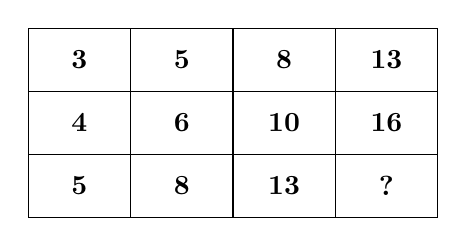
\begin{tikzpicture}
\def\w{1.3}
\def\h{0.8}
\foreach \j in {0,...,2} {
    \foreach \i in {0,...,3} {
        \draw (\i*\w, -\j*\h) rectangle (\i*\w+\w, -\j*\h+\h);
    }
}
\node at (0.5*\w, 0.5*\h) {\textbf{3}};
\node at (1.5*\w, 0.5*\h) {\textbf{5}};
\node at (2.5*\w, 0.5*\h) {\textbf{8}};
\node at (3.5*\w, 0.5*\h) {\textbf{13}};
\node at (0.5*\w, -0.5*\h) {\textbf{4}};
\node at (1.5*\w, -0.5*\h) {\textbf{6}};
\node at (2.5*\w, -0.5*\h) {\textbf{10}};
\node at (3.5*\w, -0.5*\h) {\textbf{16}};
\node at (0.5*\w, -1.5*\h) {\textbf{5}};
\node at (1.5*\w, -1.5*\h) {\textbf{8}};
\node at (2.5*\w, -1.5*\h) {\textbf{13}};
\node at (3.5*\w, -1.5*\h) {\textbf{?}};
\end{tikzpicture}
\end{varwidth}

\end{document}
